\section{AssaultCube}
Para el actual proyecto se necesita un groupware al cu\'al se le pueda acoplar la arquitectura, en este caso el sistema elegido es un video juego colaborativo de disparos en primera persona, \textit{AssaultCube}. Este groupware en particular tiene las caracter\'isticas de ser distribuido y s\'incrono seg\'un la clasificaci\'on de Ellis  	\cite{ellis1991groupware}, contiene varios tipos de elementos y los modos multijugador son entre equipos en los cuales se requiere de una buena colaboraci\'on para cumplir los objetivos de la actividad, el juego cuenta con un servidor y varios clientes que se conect\'an a \'el para jugar, la arquitectura tendr\'a que estar acoplada al servidor ya que este es el que recibe toda la informaci\'on de las actividades de los clientes.

El servidor del video juego \textit{AssaultCube}(Figura \ref{gw:asscb}) est\'a desarrollado para la plataforma Linux, el cliente para Windows, y la arquitectura a desarrollar ser\'a programada en C\#. \textit{Assault Cube} tiene diferentes modos de juego, entre ellos capturar la bandera, cuyo objetivo es llegar a la base enemiga y recuperar la bandera que est\'a ah\'i para regresarla a la propia bas; otro modo de juego es rey de la colina, que tiene por objetivo mantenerse m\'as tiempo en una posici\'on marcada por el juego que el equipo contrario; hay m\'as formas de juego adem\'as de estas dos, y en cada una de ellas las actividades son diferentes y poseen objetivos diferentes, sin embargo pueden compartir interacciones como eliminar a un enemigo por ejemplo. 

\begin{figure}[h!]
\centering
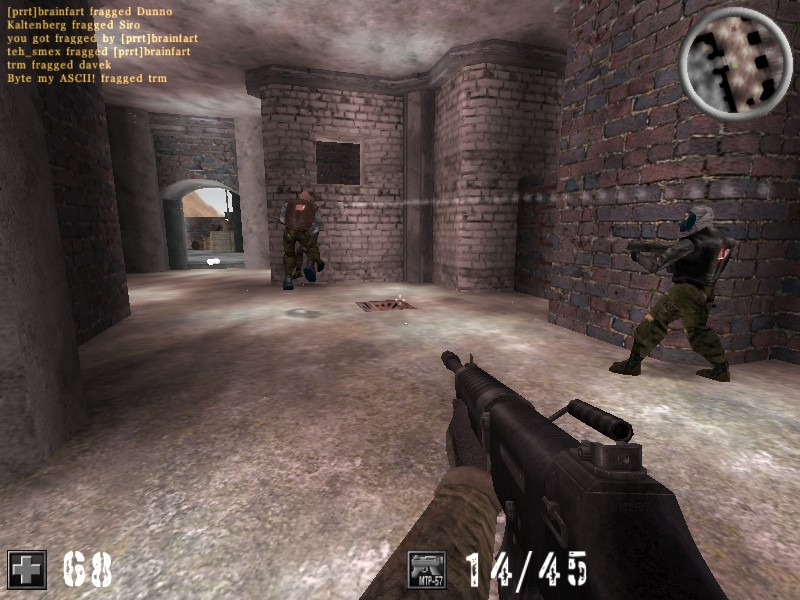
\includegraphics[scale=.25]{images/assaultcube}
\caption{Assault Cube}
\label{gw:asscb}
\end{figure}

En el Cuadro \ref{sc:interacciones} se muestran las interacciones identificadas en el juego para la actividad relacionada al modo de juego de capturar la bandera, estas interacciones est\'an relacionadas directamente con las actividades que se pueden llevar a cabo en el groupware, las interacciones se vuelven irrelevantes cuando no tienen conexi\'on con ninguna actividad, por ejemplo las interacciones del usuario con elementos de configuraci\'on en este caso particular, como en la interacci\'on \textit{"Jugador elige modo de juego"}. En estas interacciones se encuentran algunos elementos del modelo como pueden ser Actores, Tareas y Objetos,  esto nos da la pauta para empezar a dise\~nar nuestro modelo.

\begin{center}
\begin{longtable}{|p{5cm}|p{8cm}|}

\caption{Interacciones detectadas en \textit{Assault Cube}}
\label{sc:interacciones}\\
\hline
\textbf{Interacci\'on} & \textbf{Elementos identificados}\\
\hline
\endfirsthead
\multicolumn{2}{c}%
{\tablename\ \thetable\ -- \textit{... Contin\'ua de p\'agina anterior}} \\
\hline
\textbf{Interacci\'on} & \textbf{Elementos identificados} \\
\hline
\endhead
\hline \multicolumn{2}{r}{\textit{Contin\'ua en siguiente p\'agina...}} \\
\endfoot
\hline
\endlastfoot
\textbf{Jugador se Mueve} & Actor: Jugador; Tarea: Moverse\\\hline

\textbf{Jugador salta} & Actor: Jugador; Tarea: Saltar\\\hline

\textbf{Jugador dispara arma} & Actor: Jugador; Tarea: Saltar; Objeto: Arma\\\hline

\textbf{Jugador recarga arma} & Actor: Jugador; Tarea: Recargar; Objeto: Arma\\\hline

\textbf{Jugador dispara arma} & Actor: Jugador; Tarea: Saltar; Objeto: Arma\\\hline

\textbf{Jugador cambia arma} & Actor: Jugador; Tarea: Cambiar; Objeto: Arma\\\hline

\textbf{Jugador obtiene mejora de salud} & Actor: Jugador; Tarea: Obtener; Objeto: Mejora de salud\\\hline

\textbf{Jugador obtiene protecci\'on} & Actor: Jugador; Tarea: Obtener; Objeto: Protecci\'on\\\hline

\textbf{Jugador obtiene munici\'on} & Actor: Jugador; Tarea: Obtener; Objeto: munici\'on\\\hline

\textbf{Jugador envia mensaje de texto} & Actor: Jugador; Tarea: enviar; Objeto: Mensaje de texto\\\hline

\textbf{Jugador envia mensaje de voz predefinido} & Actor: Jugador; Tarea: enviar; Objeto: Mensaje de voz\\\hline

\textbf{Jugador elige arma inicial} & Actor: Jugador; Tarea: Elegir; Objeto: Arma predeterminada\\\hline

\textbf{Jugador cambia rol} & Actor: Jugador; Tarea: Cambiar; Objeto: Rol\\\hline

\textbf{Jugador se agacha} & Actor: Jugador; Tarea: Agacharse\\\hline

\textbf{Jugador se suicida} & Actor: Jugador; Tarea: Suicidarse\\\hline

\textbf{Jugador es eliminado} & Actor: Jugador; Tarea: Ser eliminado\\\hline

\textbf{Jugador elimina oponente} & Actores: JugadorA, JugadorB; Tarea: Eliminar\\\hline

\textbf{Jugador reaparece} & Actor: Jugador; Tarea: Reaparecer\\\hline

\textbf{Jugador captura bandera} & Actor: Jugador; Tarea: Capturar; Objeto: Bandera\\\hline

\textbf{Jugador regresa bandera a su base} & Actor: Jugador; Tarea: Recuperar; Objeto: Bandera \\\hline

\textbf{Jugador ve mapa} & Actor: Jugador; Tarea: Ver; Objeto: Mapa\\\hline

\textbf{Jugador ve puntuaciones} & Actor: Jugador; Tarea: Ver; Puntuaciones\\\hline

\end{longtable}
\end{center}

En la lista anterior se identifican algunos elementos del modelo del groupware, por ejemplo, jugador como actor; arma, munici\'on y mapa como posibles objetos, y el conjunto de ellos asociados a una tarea; tambi\'en de ser necesario se pueden tomar en cuenta tareas como \textit{bloquear arma} o \textit{mostrar posici\'on en el mapa} que podr\'an ser utilizadas como resultado para los guiones de comportamiento explicados m\'as adelante. Adem\'as de los elementos identificados por medio de la observaci\'on, se explor\'o el sitio web oficial de la aplicaci\'on \cite{assCube2014} para extraer m\'as informaci\'on del juego. Se encontraron dos \textbf{Equipos}: team clubers liberation army(TCLA) y rabid viper special forces(RVSF) los que compiten uno en contra del otro en cada partida. Dos tipos de \textbf{objetos}, armas y art\'iculos, para las armas se describen atributos como tiempo de recarga, capacidad de munici\'on, rafaga de disparo, etc. Para los art\'iculos s\'olo se define el atributo de tiempo de reaparici\'on. Tambi\'en se identificaron \textbf{objetivos} seg\'un los tipos de partida, de los que se infieren algunas \textbf{metas}. En el Cuadro \ref{sc:dominio} se muestran los elementos de dominio que se identificaron mediante la revisi\'on de la documentaci\'on del sistema.

\begin{center}
\label{sc:dominio}
\begin{longtable}{|p{3cm}|p{9cm}|}

\caption{Elementos de dominio de \textit{Assault Cube}}\\
\hline
\textbf{Elemento de Meta modelo} & \textbf{Elemento de dominio de la aplicaci\'on}\\
\hline
\endfirsthead
\multicolumn{2}{c}%
{\tablename\ \thetable\ -- \textit{... Contin\'ua de p\'agina anterior}} \\
\hline
\textbf{Elemento de Meta modelo} & \textbf{Elemento de dominio de la aplicaci\'on} \\
\hline
\endhead
\hline \multicolumn{2}{r}{\textit{Contin\'ua en siguiente p\'agina...}} \\
\endfoot
\hline
\endlastfoot

Actores & Jugador(p.ej. Juan, Ana, Marcos, etc.)\\
\hline Equipos & Team Clubers Liberation Army (TCLA);
Rabid Viper Special Forces (RVSF).\\
\hline Objetos & Armas , Art\'iculos. \\
\hline Roles & Explorer, Protector, Fragger, Recoverer.\\
\hline Objetivos & capturar la bandera, robar la bandera enemiga, eliminar jugadores enemigos, regresar la bandera a la base aliada.\\
\hline Metas & Tener la mayor cantidad de puntos, eliminar mayor n\'umero de enemigos, sobrevivir la mayor cantidad de tiempo.\\
\hline Actividades & Capturar la bandera en equipo, Juego a muerte.

\end{longtable}
\end{center}

Con estos elementos se instanci\'o el modelo de dominio en base de datos, el modelo resultante es representado en la Figura \ref{fig:DomModel}.
\newpage
\begin{figure}[h]
\centering
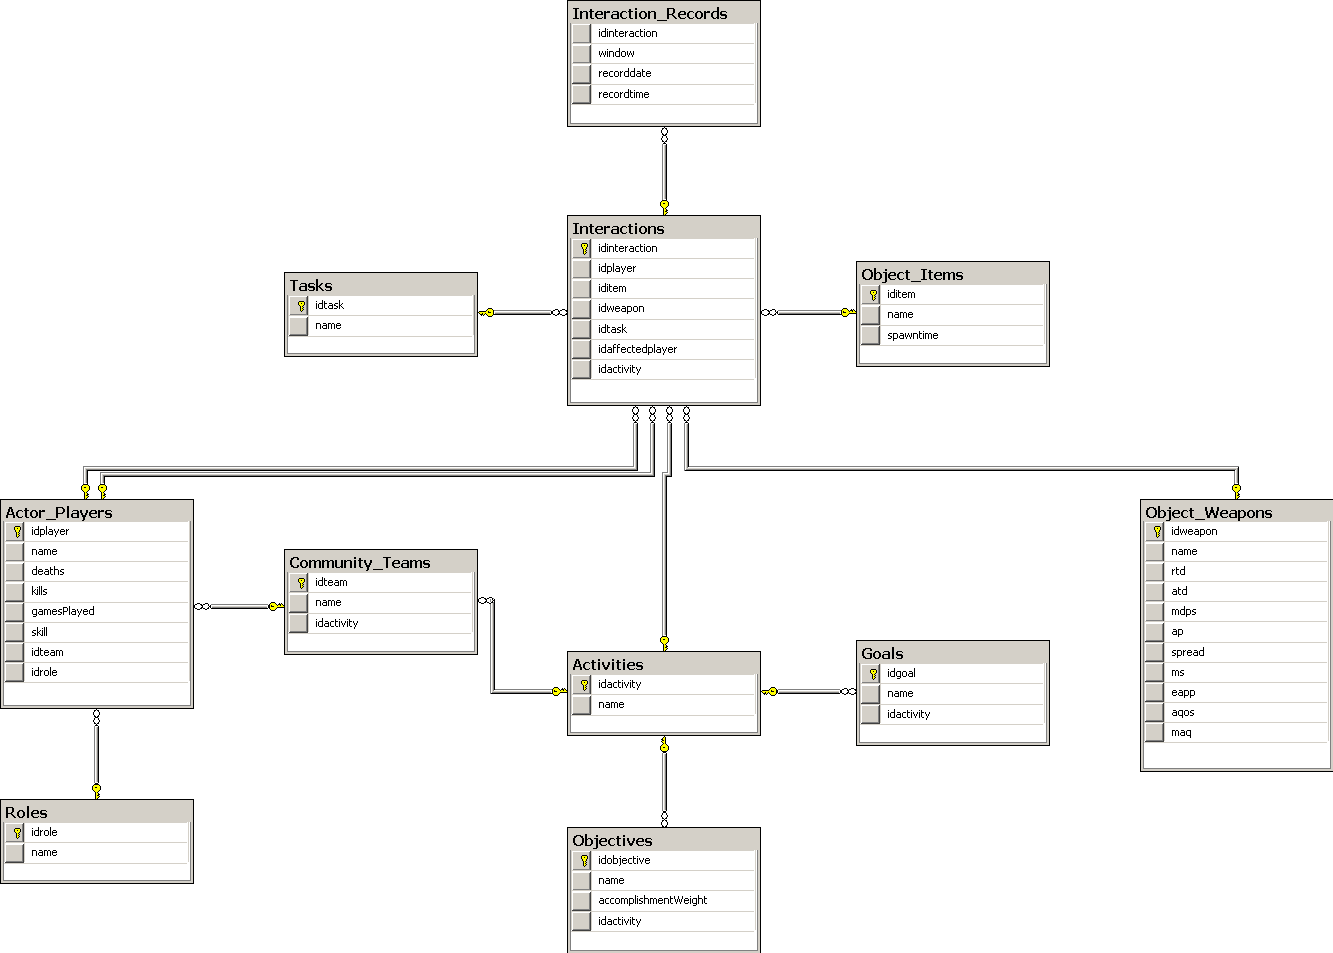
\includegraphics[width=0.7\linewidth]{images/GameModelDiagram}
\caption{Modelo de dominio de \textit{Assault Cube}}
\label{fig:DomModel}
\end{figure}

Despu\'es de instanciar el modelo de aplicaci\'on se agregaron datos para fines de pruebas, se tom\'o  como punto inicial la actividad '\textit{TeamKeepTheFlag}' a la cual se le agrag\'o la meta '\textit{scoreTheMost}' y equipos, a su vez a a las metas se le asocian objetivos y a estos tareas; de manera similar a los equipos le son asociados actores, la jerarqu\'ia de estas instancias se puede ver en la Figura\ref{fig:instanciaActividad}

\begin{figure}[h]
\centering
\includegraphics[width=0.7\linewidth]{./images/instanciaActividad}
\caption{Instancias para caso de estudio}
\label{fig:instanciaActividad}
\end{figure}


A partir de estos elementos pueden empezar a definirse algunas reglas, por ejemplo establecer una regla que diga que si un jugador captur\'o una bandera y est\'a en peligro inminente de ser atacado, el sistema muestre a sus compa\~neros de equipo la ubicaci\'on del abanderado y env\'ie una se\~nal de auxilio para que ellos puedan acudir a su ayuda.

Con estas interacciones y el conjunto de reglas definido se propone un conjunto de guiones que describen diferentes tipos de comportamiento dado el caso de estudio; entre los que se encuentra un guion para jugadores novatos, un guion para jugadores in\'utiles, uno para jugadores con comportamiento sospechoso que podr\'ian considerarse como traidores y uno para jugadores expertos. Estos guiones servir\'an al momento de ejecutar, los guiones se definen como sigue.

\begin{table}[h!]
\caption{Gui\'on para jugador inactivo}
\label{guion:inactive}
\centering
\begin{tabular}{|p{10cm}|c|}
\hline \textbf{Regla} & \textbf{Frecuencia} \\
\hline $Actor(Player\{*\})-Task(Shot)$ & 3 \\
\hline \& $Actor(Player\{*\})-Task(Move)$ & 10 \\
\hline \& $Actor(Player\{*\})-Task(PickItem)$ & 5\\ 
\hline \& $Actor(Player\{*\}).enemyKills=0$ & no aplica\\
\hline\& $Actor(Player\{*\}).allyKills=0$ & no aplica\\
\hline\& $Actor(Player\{*\})-Task(captureFlag)$ & 1\\
\hline\& $Actor(Player\{*\}).socialPresense=bad$ & no aplica\\
\hline\& $Actor(Player\{*\}) \rightarrow Team(red)$  & no aplica\\
\hline \multicolumn{2}{c}{$:=$} \\
\hline $[Actor(Player\{*\})  \rightarrow Team(red)]-Task(sendWarningMessage, Object(UI\{messageConsole\})$ & no aplica\\
\hline

\end{tabular}
\end{table}

El guion de jugador inactivo del Cuadro   \ref{guion:inactive} describe el comportamiento de un jugador con poca participaci\'on en las partidas, se definen tareas relativas a la actividad del jugador como disparar con frecuencias m\'inimas que se tienen que cumplir para poder decir que ese jugador es poco activo, tambi\'en se comparan algunos de sus atributos como el n\'umero de enemigos que el jugador ha eliminado, en este caso es cero, como resultado a este comportamiento se manda a ejecutar una tarea que muestra un mensaje de advertencia a los compa\~neros del jugador indic\'andoles sobre su comportamiento para que puedan tomar las medidas necesarias.

\begin{table}[h!]
\caption{Gui\'on para jugador novato}
\label{guion:rookie}
\centering
\begin{tabular}{|p{10cm}|l|}
\hline \textbf{Regla} & \textbf{Frecuencia} \\
\hline $Actor(Player\{*\}).enemyKills<2$ & no aplica\\
\hline \& $Actor(Player\{*\}).deads>2$ & no aplica\\
\hline \& $Actor(Player\{*\})-Task(Shot)$ & 5\\
\hline \& $Actor(Player\{*\})-Task(scoreCapturedFlag)$ & 1\\
\hline \& $Actor(Player\{*\})-Task(loseFlag)$ & 1\\
\hline \& $[Actor(Player\{*\}) \rightarrow Team(red)]-Task(Shot).Success = true$ & 5\\
\hline \& $[Actor(Player\{*\}) \rightarrow Team(red)]-Task(Shot).Dimension = positive$ & 5\\
\hline \multicolumn{2}{l}{$:=$} \\
\hline $[Actor(Player\{*\}) \rightarrow Team(red)]-Task(sendMessage, Object(UI\{messageConsole\})$ & no aplica\\
\hline
\end{tabular}
\end{table}

Para que un jugador sea considerado como novato, se tomaron en cuanta el n\'umero de muertes enemigas que ha causado el jugador en un intervalo de tiempo, que haya capturado la bandera al menos una vez, y que los disparos que haya hecho sean efectivos con cierta frecuencia. Este gui\'on es descrito en el Cuadro \ref{guion:rookie}.

\begin{table}[h!]
\caption{Guion para jugador experto}
\label{guion:expert}
\centering
\begin{tabular}{|p{10cm}|l|}
\hline \textbf{Regla} & \textbf{Frecuencia} \\
\hline $Actor(Player\{*\}).enemyKills>5$ & no aplica\\
\hline \& $[Actor(Player\{*\}) \rightarrow Team(red)]-Task(Shot).Success = true$ & 5\\
\hline \& $[Actor(Player\{*\}) \rightarrow Team(red)]-Task(Shot).Dimension = positive$ & 5\\
\hline \& $[Actor(Player\{*\}) \rightarrow Team(red)]-Task(Destroy).Bearer = true$ & 1\\
\hline \& $Actor(Player\{*\})-Task(captureFlag)$ & 3\\
\hline \& $Actor(Player\{*\}).socialPresence=quite good$ & no aplica\\
\hline \& $Actor(Player\{*\}).deads<2$ & no aplica\\
\hline\multicolumn{2}{l}{$:=$}\\
\hline $[Actor(Player\{*\}) \rightarrow Team(red)]-Task(showPosition,Object(UI\{map\})$ & no aplica\\
\hline \& $[Actor(Player\{*\}) \rightarrow Team(red)]-Task(sendHelpMessage,Object(UI\{messageConsole\})$ & no aplica\\
\hline
\end{tabular}
\end{table}

El gui\'on mostrado en el Cuadro \ref{guion:expert} especifica el comportamiento de un jugador que tiene experiencia jugando el juego, para esto se mide la cantidad de enemigos eliminados haci\'endose efectivo para m\'as de 5 muertes en un lapso de tiempo dado, adem\'as se cuentan las veces que el jugador ha capturado una bandera o ha marcado puntos, y al igual que el jugador inactivo se mide su presencia social la cual tiene que ser alta para ser considerado un jugador experto. Como resultado al cumplimiento de este gui\'on se activa la posici\'on de este jugador experto en el mapa, y avisa a los dem\'as que se mantengan cerca de \'el para que se apoyen mutuamente.

\begin{table}[h!]
\caption{Guion de jugador traidor}
\label{guion::traitor}
\centering
\begin{tabular}{|p{10cm}|l|}
\hline $Actor(Player\{*\})-Task(captureFlag)$ & 1\\
\hline \& $[Actor(Player\{*\})\rightarrow Team(RVSF)]-Task(Shot)-Affects([Actor(Player\{*\})->Team(red)])$ & 3\\
\hline \& $Actor(Player\{*\}).socialPresence = bad$ & no aplica\\
\hline \& $Actor(Player\{*\}).allyKills > 2$ & no aplica\\
\hline \& $[Actor(Player\{*\})\rightarrow Team(RVSF)]-Task(Shot).outcome > 0$ & 0\\
\hline \multicolumn{2}{l}{$:=$}\\
\hline $[Actor(Player\{*\})\rightarrow Team(RVSF)]-Task(blockWeaponry,Object(Weapon\{*\})$ & no aplica\\
\hline \& $[Actor(Player\{*\})\rightarrow Team(RVSF)]-Task(sendWarningMessage,Object(UI\{messageConsole\})$ & no aplica\\
\hline
\end{tabular}
\end{table}

Por \'ultimo se define un gui\'on(Cuadro  \ref{guion::traitor}) para un jugador cuyo comportamiento afecta a los miembros del mismo equipo, como disparos a sus compa\~neros, tambi\'en se mide el n\'umero de disparos que hizo contra enemigos si son menores o igual a uno entonces ese jugador se considera un traidor, y como medidas computacionales se env\'ia la tarea de bloquear armamento y un mensaje a sus aliados donde se avise de su comportamiento para que tomen la estrateg\'ia adecuada.

\section{Prototipo}


El prototipo de la arquitectura, mostrado en la Figura \ref{imp:Implementacion}, sigue la misma estructura que el dise\~o conceptual dividido en tres capas: recuperaci\'on de datos, gestion de datos y uso contextual. En la capa de recuperaci\'on de datos se encuentran dos tipos de servicios, los que reciben las tareas ejecutadas en la aplicaci\'on colaborativa, en este caso \textbf{\textit{AssaultCube}}, y los que recibe actualizaciones del estado de los elementos que participan en las actividades llevadas a cabo en el groupware.

En la capa de gesti\'on de datos  se implementan dos servidores, SQL Server como motor de base de datos e Internet Information Services 7 (IIS7) como servidor web. Dentro del servidor de base de datos se encuentra el  modelo conceptual y los modelos de dominio que se generen; dentro del servidor web se encuentran las aplicaciones necesarias para definir e instanciar los modelos y servicios usados para recibir los datos durante la ejecuci\'on de \textit{AssaultCube}, la primera aplicaci\'on es la Plataforma web de Definici\'on de Dominio de Aplicaci\'on(\textbf{PDDA})  programada en el marco de trabajo de ASP.NET. Dentro de esta aplicaci\'on se encuentran formularios para definir elementos del dominio y para el registro de nuevos casos de estudio, los elementos definidos se almacenan para que puedan ser reutilizados en otro casos de estudio; tambi\'en cuenta con un m\'odulo para definir los guiones de comportamiento, en este se escriben las reglas para cada guion y son validadas por un parser en la capa de uso de contexto. La segunda aplicaci\'on es un m\'odulo programado en el lenguaje C$\sharp$ con la plataforma .NET versi\'on 4.0.0,  que genera las instancias del modelo definido en la plataforma implementando t\'ecnicas de programaci\'on reflexiva, una de las instancias es la del modelo de dominio en el servidor de base de datos, otra es el modelo de clases y el tercero son los servicios propios del dominio en el servidor web IIS7. 

Dentro de la capa de uso de contexto se encuentran el int\'erprete de las reglas usado por la plataforma web y el motor de inferencia que es el objeto principal de este trabajo, este motor accede al modelo de dominio en la base de datos para recuperar los guiones de comportamiento, crear los objetos relativos a los guiones y verificarlos cada vez que se reciben ejecuciones de tareas desde \textit{AssaultCube}, cuando el motor detecta que un gui\'on se cumple recupera las tareas resultantes descritas en dicho gui\'on y un servicio de resultados lo env\'ia al groupware para su interpretaci\'on y ejecuci\'on. 

\begin{figure}[h]
\centering
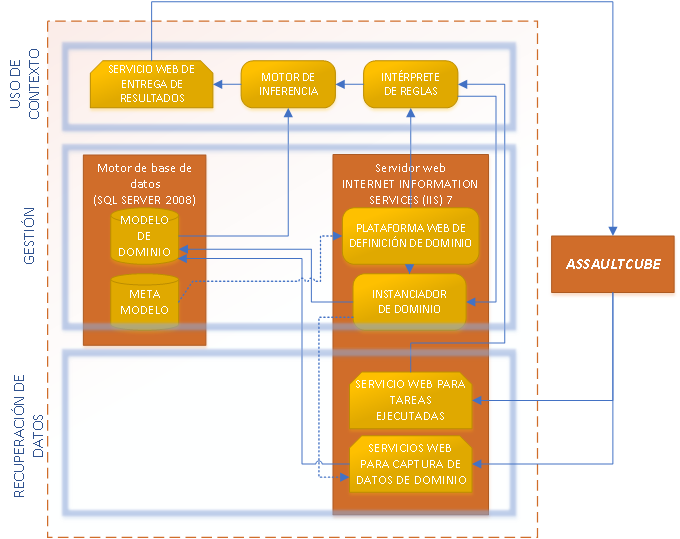
\includegraphics[width=0.7\linewidth]{images/arquitecturaImplementacion}
\caption{Arquitectura de implementaci\'on}
\label{imp:Implementacion}
\end{figure}

\section{Int\'erprete de reglas y Motor para de inferencia de guiones de comportamiento}

Para el presente trabajo se proponen un lenguaje, validado por un int\'erprete, dise\~ado para describir las interacciones que se llevan a cabo en una actividad y las condiciones que se deben de cumplir para asumir que un usuario tiene un comportamiento en particular.

Para el int\'erprete se implement\'o una gram\'atica libre de contexto asociada a la estructura de los diferentes tipos de reglas propuestas, esta gram\'atica es la siguiente:

\begin{verbatim}


S->ML:=XJ       //Elemento      //Pertenencia
M->P            E->m(e{iH})     P->EOE
M->C            E->m(*)         O->->
M->X            E->m(e{*})      O->~>
J->&XJ          E->m(iH)            
J->$            H->,iH              
L->&ML          H->$                
L->$            

//Comparacion   //ejecucion de tareas
C->E.aKv        X->F-t(n,F)Q
K->=            X->F-t(n)Q
K->~            Q->.aKv
K-><            Q->$
K->>            F->E
\end{verbatim}

A partir de esta gram\'atica se implementa un aut\'omata SLR en el lenguaje C$\sharp$ usando la plataforma .NET versi\'on 4.0,  \'este determina a validez sint\'actica de una regla. Antes de este proceso se verifica con expresiones regulares que las reglas cumplan con el patr\'on de los tipos de reglas definido, este an\'alisis regresa como resultado una serie de car\'acteres que despu\'es son an\'alizados por el aut\'omata.

El motor de inferencia tambi\'en es implementado en el lenguaje C$\sharp$ bajo la plataforma .NET 4.0, b\'asicamente el motor recupera los guiones de la base de datos del dominio de la aplicaci\'on y  los utiliza como lista de verificaci\'on para revisar la frecuencia de las tareas definidas en los guiones, teniendo tambi\'en la opci\'on de ejecutar los guiones verificando que las tareas descritas s\'olo se ejecuten una s\'ola vez. El pseudoc\'odigo de el motor es el siguiente:

\begin{verbatim}
recuperar scripts
    instanciar scrpits
        recuperar tareas
        recuperar comparaciones
        recuperar pertenencias
    mientras corrida de juego
        recibir tarea
        buscar tarea en cada uno de los scripts
        si tarea esta en script 
            decrementar contador
            si contador de todas las tareas == 0
                verificar reglas de comparacion
                verificar pertenencias
                si ambas son verdaderas
                    regresar tareas resultantes
                    reiniciar contadores de tareas
\end{verbatim}

Para probar el motor se almacenaron los siguientes guiones con sus reglas en la base de datos(Figura \ref{fig:instanciasPrueba}).

\begin{figure}
\centering
\includegraphics[width=0.7\linewidth]{./images/instanciasPrueba}
\caption{Datos de los guiones almacenados}
\label{fig:instanciasPrueba}
\end{figure}

El motor es alimentado por cadenas en formato de tareas ejecutadas por cada una de las cuales decrementa un contador en los guiones como se muestra en la Figura\ref{fig:scripts}

\begin{figure}
\centering
\includegraphics[width=0.9\linewidth]{./images/scripts}
\caption{Conteo de tareas ejecutadas en los guiones}
\label{fig:scripts}
\end{figure}

El motor se puede correr de dos formas distintas, una en la que toma en cuenta las frecuencias definidas, y otra en la que cada tarea s\'olo necesita ejecutarse una vez para que el guion se cumpla.
Cuando los contadores de alg\'un guion llegan a cero en las frecuencias de las tareas este valida las dem\'as condiciones del guion y regresa las tareas a ejecutar en el groupware como respuesta como se muestra en la Figura \ref{fig:ScriptMatch}

\begin{figure}[h]
\centering
\includegraphics{./images/ScriptMatch}
\caption{Tarea regresada cuando el guion de prueba se cumple}
\label{fig:ScriptMatch}
\end{figure}
